\chapter{Experimental Setup} \label{Chapter4}

\section{RAC components} \label{RAC components}
In order to provide a solution to the goals stated in Section \ref{Business context} it is important to obtain a good understanding of all aspects that play a role within the RAC. A short description of all hardware and software aspects is given below. It is possible that not all described components are relevant to this project. Nevertheless, some terms may be used throughout this thesis and therefore a brief description of these components can be helpful. Section \ref{Hardware} gives an overview of the hardware components within the RAC, the robotic arm, vision camera and any feeder. The robotic arm will be discussed more thoroughly because that aspect requires the most maintenance and is therefore more interesting. Section \ref{Software} gives an overview of all software components within the RAC, V+\textsuperscript{\tiny{TM}}, ACE\textsuperscript{\tiny{TM}}, and AdeptSight\textsuperscript{\tiny{TM}} that play a role by designing the CBM tool.

\subsection{Hardware} \label{Hardware}
As mentioned before, the RAC consist of several components (anyfeeder, vision camera, robotic arm, conveyor belt). The vision cameras and the robotic arms are products of Bremer Werk für Montagesysteme (BWM), a company that produces assembly systems, automation systems, and special-purpose machine manufacturing\footnote{https://www.bwm-gmbh.de/en/unternehmen/}. BWM has established the ALs at Philips by installing the RACs and providing controllers to the components. For example, the trajectory that a robotic arm has to execute in order to assemble certain parts of a shave is programmed by BWM. 

The vision guidance system and Adept AnyFeeder\textsuperscript{\tiny{TM}} that are part of RB34 are not discussed in detail. Obtaining data from the anyfeeder is a complex task that should be performed by Adept programmers and will be outside the scope of this project. Maintenance on the vision guidance system is rare and therefore it is not relevant to predict it.  

The robotic arms within RAC RB34 that are used to assemble the shaver units are Adept Cobra s600's with four axis. This is a high-performance Selective Compliance Assembly Robot Arm (SCARA) robot system for mechanical assembly, material handling, packaging, machine tending, screw driving, and other applications that require fast and precise automation. This robot include the Adept SmartController EX\textsuperscript{\tiny{TM}} motion controller, an ultra-compact, high-performance, distributed robot motion controller capable of controlling an entire production line managing multiple robots. Before this project, RB34 featured a Smart Controller CX\textsuperscript{\tiny{TM}} which is not able to subtract the data from the RAC due to complex programming issues. Therefore, Smart Controller EX, a newer version motion controller from adept, is installed on RB34 especially for this project. In Figure \ref{fig:Cobra s600} and \ref{fig:SmartController} the robot arm and the motion controller are depicted, respectively, and a full description of the hardware is available on the website of Adept\footnote{http://www.adept.com/products/robots}.
\begin{figure}[ht]
\centering
\begin{subfigure}[b]{0.49\textwidth}
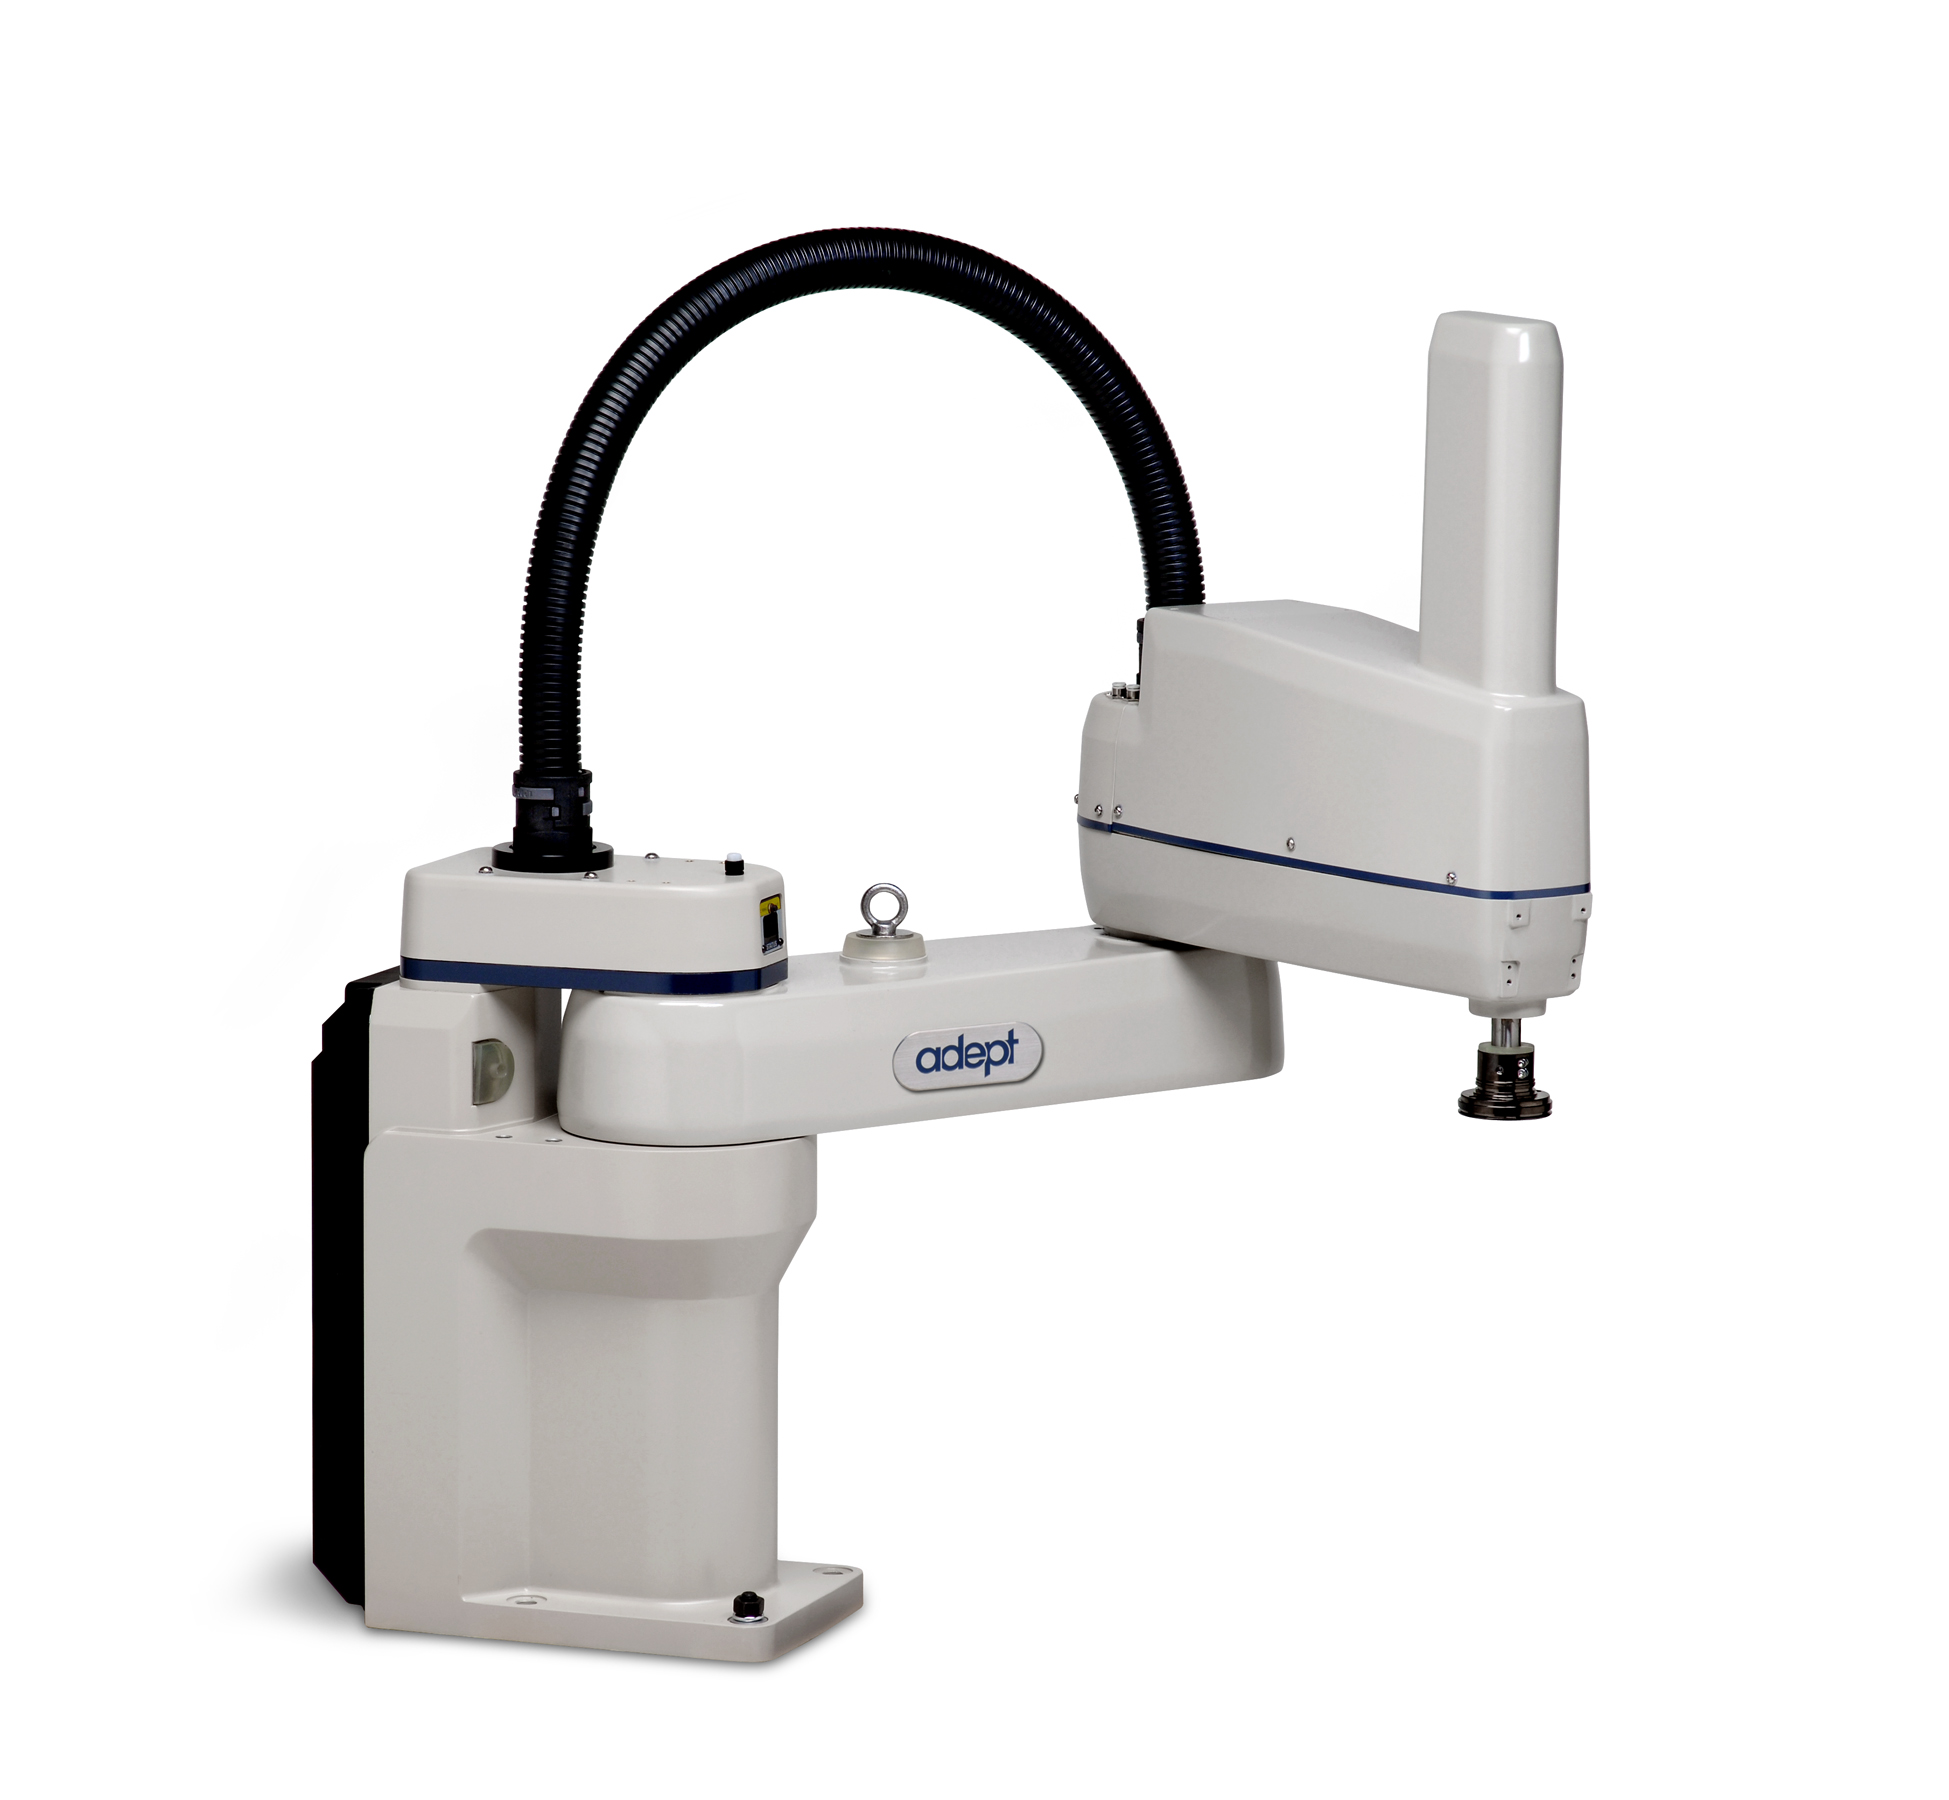
\includegraphics[width=\textwidth]{Figures/Cobra-600}
\caption{Adept Cobra s600}
\label{fig:Cobra s600}
\end{subfigure}
\begin{subfigure}[b]{0.49\textwidth}
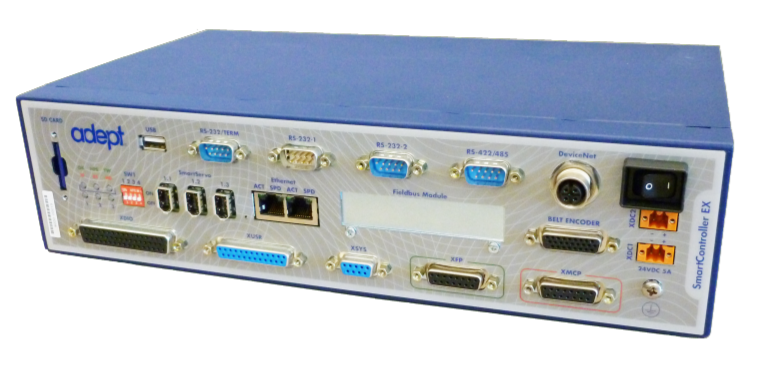
\includegraphics[width=\textwidth]{Figures/SmartController}
\caption{Adept SmartController EX}
\label{fig:SmartController}
\end{subfigure}
\caption[Relevant hardware components of RB34]{Hardware components of RB34}
\label{fig:HardwareComponents}
\end{figure}

\subsection{Software} \label{Software}
The programming language that is used is V+, a language to provide an integrated solution to all of the programming needs in a robotic workcell, including safety, robot motion, vision operations, force sensing and I/O. It is used to combine the vision guidance software with the control software that is installed on the PC of the RAC. 

AdeptSight\textsuperscript{\tiny{TM}} is an easy-to-use, standalone vision guidance and inspection package and comes complete with all the necessary accessories. The software includes a powerful framework that can be used to develop customized vision guidance and inspection applications. 

The interaction with operators at the RACs is provided by an interface called ACE (Automation Control Environment) which features an integrated environment for robot and control. Data is available for every robotic arm motor regarding temperature, torque, voltage, position error and duty cycle and can be displayed on the Human Machine Interface (HMI) which is connected with the control system of a RAC. The different types of data and their relevance are discussed in Section \ref{Data Gathering}.

\section{Data gathering} \label{Data Gathering}
In this section, data that is useful for the execution of the research will be presented. By analyzing the useful data, the relevant data to investigate can be determined research question one will be answered and research question one will be answered. Data that can be subtracted from the RAC controller is mentioned briefly. In table \ref{Data types}, all data types that can be obtained are listed. From those types of data it should be determined which type is relevant and is able to predict  maintenance. Since all Cobra s600  robots within the AL are identical and execute similar tasks, it is assumed that the same data type(s) will predict similar maintenance for all Cobra s600 robots. 

%A new table should be build to list all data types. The data types are available on http://www1.adept.com/main/ke/data/pdf_web/ace_ug.pdf. 
%\begin{table}[ht]
%\centering
%\caption[Data types available from the SmartController]{Data types available from the SmartController}
%\label{Data types}
%\begin{tabular}{l | l | l}
%\multicolumn{3}{|c|}{Data Type} \\
%\hline
%Robot Bus Voltage & Voltage \\
%Robot AC input & Root-mean-square (RMS) Voltage \\
%Robot DC input & Voltage \\
%Robot Base board temperature & $^\circ$Celsius \\
%Motor Amplifier temperature & $^\circ$Celsius \\
%Motor Duty cycle & \% limit \\
%Motor Peak torque & \% maximum torque \\
%Motor Peak velocity & Revolutions per Minute (RPM) \\
%Motor Peak position error & \% soft envelope error
%\end{tabular}
%\end{table}

\begin{table}[ht]
\centering
\caption[Data types available from the SmartController]{Data types available from the SmartController}
\label{Data types}
\begin{tabular}{l | c}
Data type & Unit \\
\hline
Robot Bus Voltage & Voltage \\
Robot AC input & Root-mean-square (RMS) Voltage \\
Robot DC input & Voltage \\
Robot Base Board temperature & $^\circ$Celsius \\
Motor Amplifier temperature & $^\circ$Celsius \\
Motor Duty cycle & \% limit \\
Motor Peak torque & \% maximum torque \\
Motor Peak velocity & Revolutions per Minute (RPM) \\
Motor Peak position error & \% soft envelope error 
\end{tabular}
\end{table}

\begin{figure}[ht]
\begin{subfigure}{.5\textwidth}
 \centering
 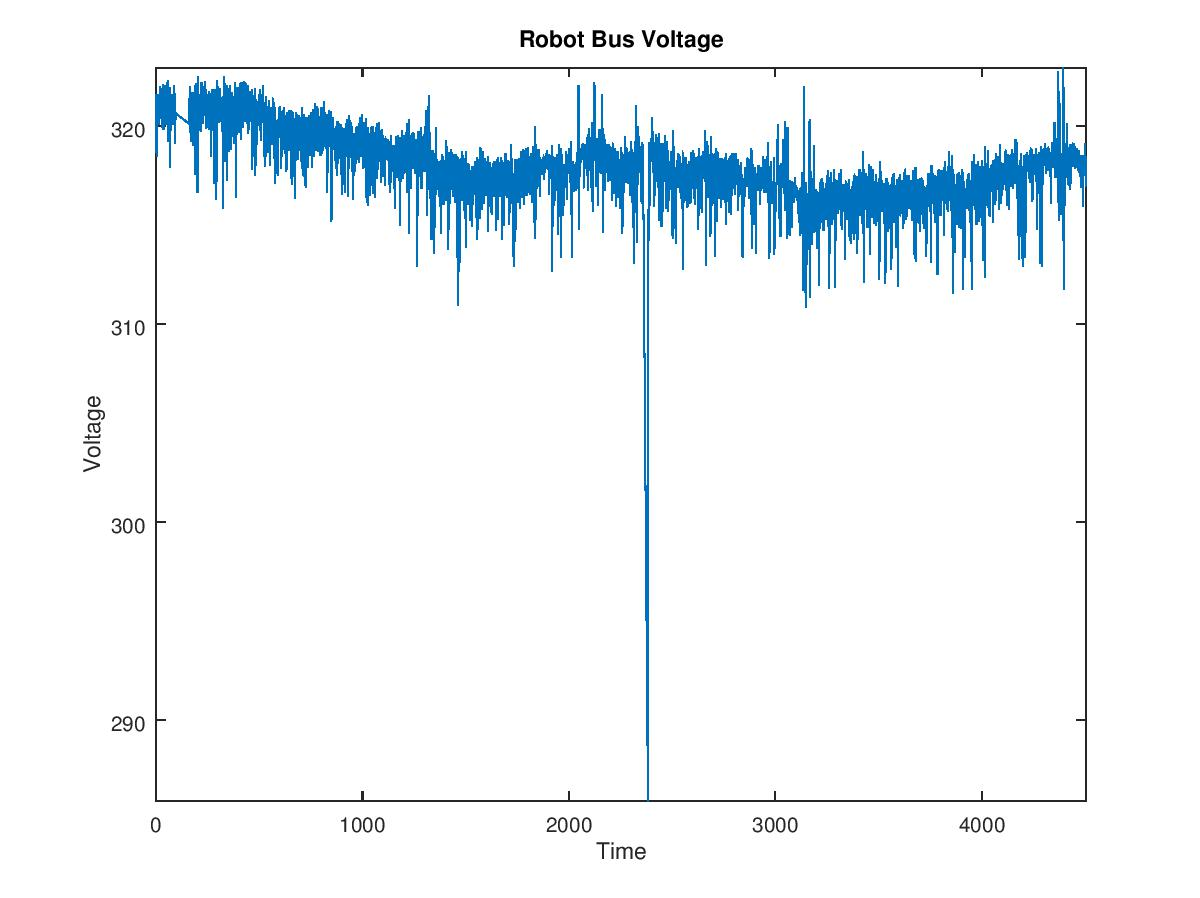
\includegraphics[width=.9\linewidth]{Figures/Robot_Bus_Voltage}
 \caption{Robot Bus Voltage}
 \label{fig:Robot Bus Voltage}
\end{subfigure}
\begin{subfigure}{.5\textwidth}
 \centering
 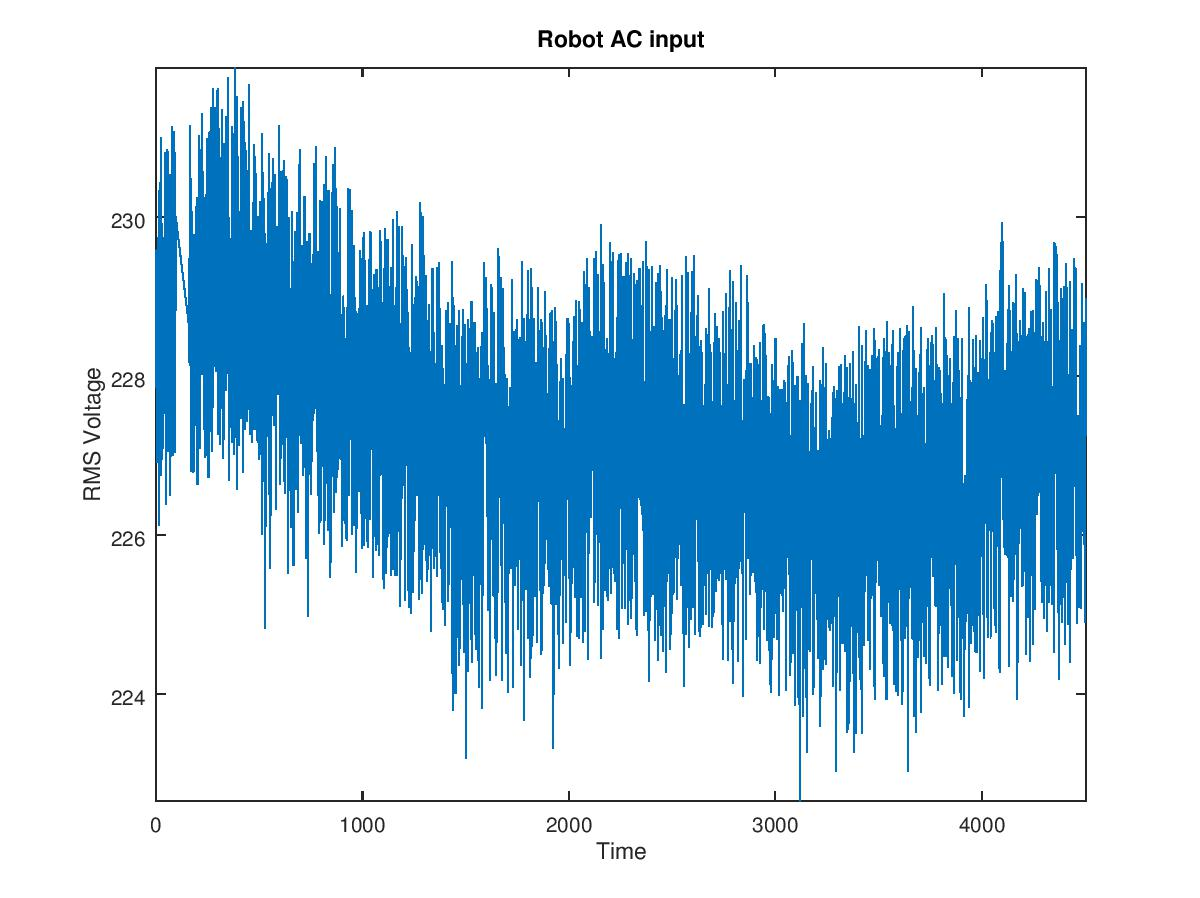
\includegraphics[width=0.9\linewidth]{Figures/Robot_AC_input}
 \caption{Robot AC input}
 \label{fig:Robot AC input}
\end{subfigure}\\
\begin{subfigure}{.5\textwidth}
 \centering
 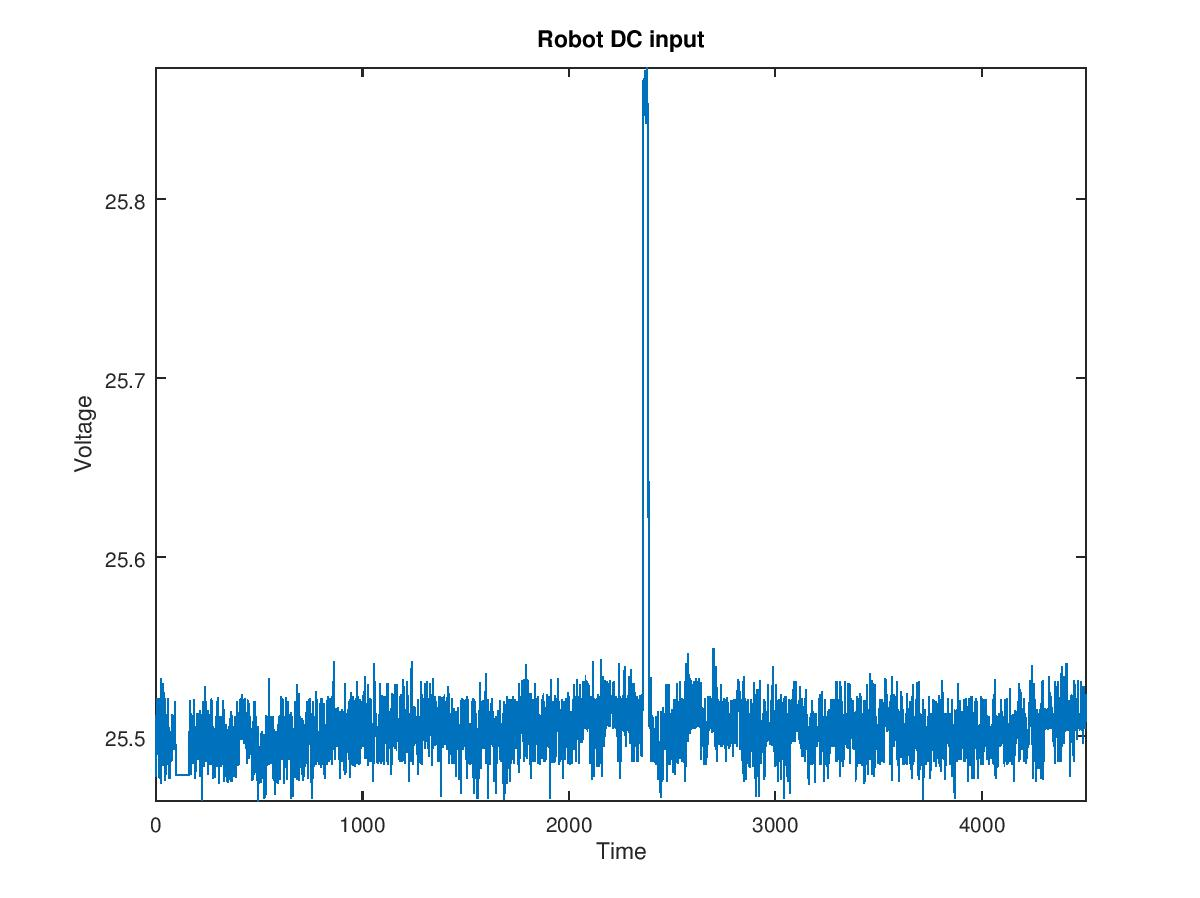
\includegraphics[width=.9\linewidth]{Figures/Robot_DC_input}
 \caption{Robot DC input}
 \label{fig:Robot DC input}
\end{subfigure}
\begin{subfigure}{.5\textwidth}
 \centering
 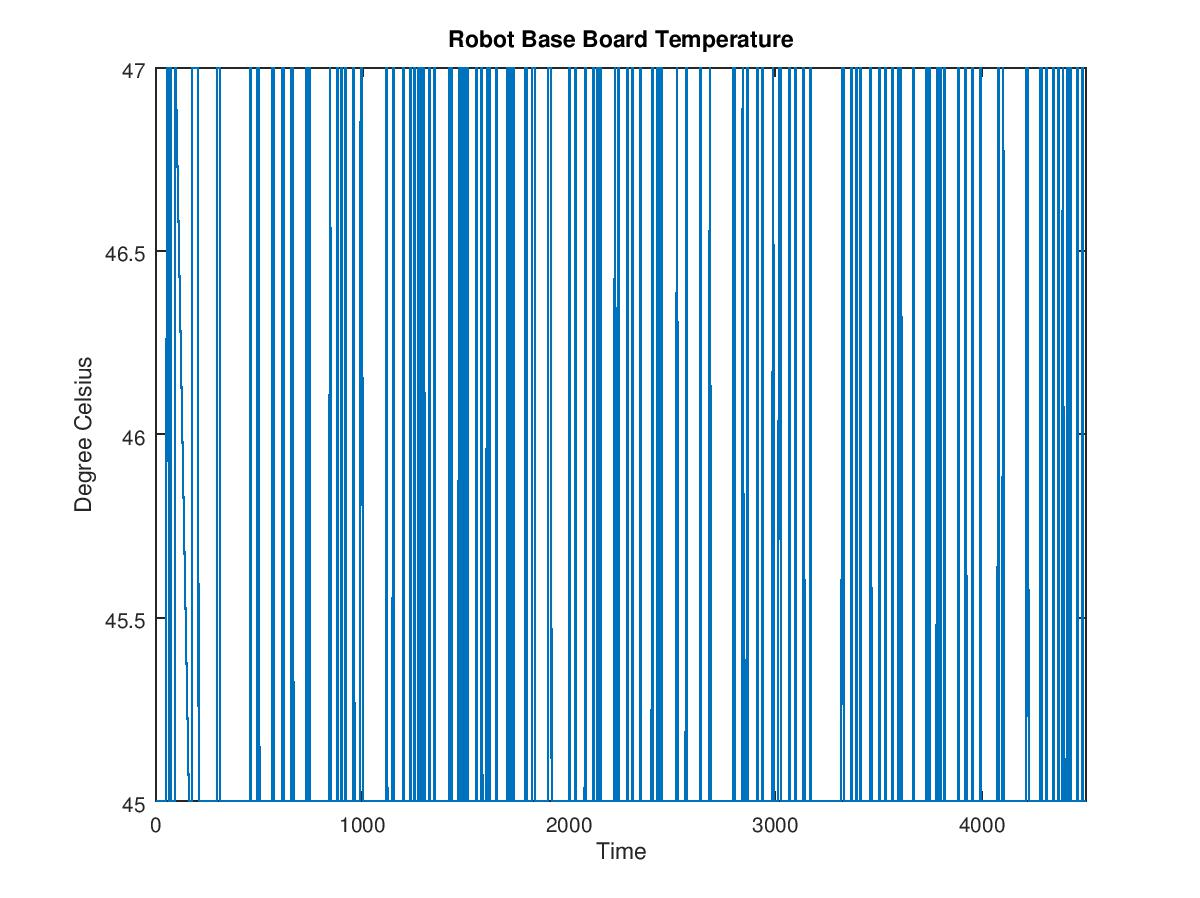
\includegraphics[width=.9\linewidth]{Figures/Robot_Base_Board_Temperature}
 \caption{Robot Base Board Temperature}
 \label{fig:Robot Base Board Temperature}
\end{subfigure}\\
\begin{subfigure}{.5\textwidth}
 \centering
 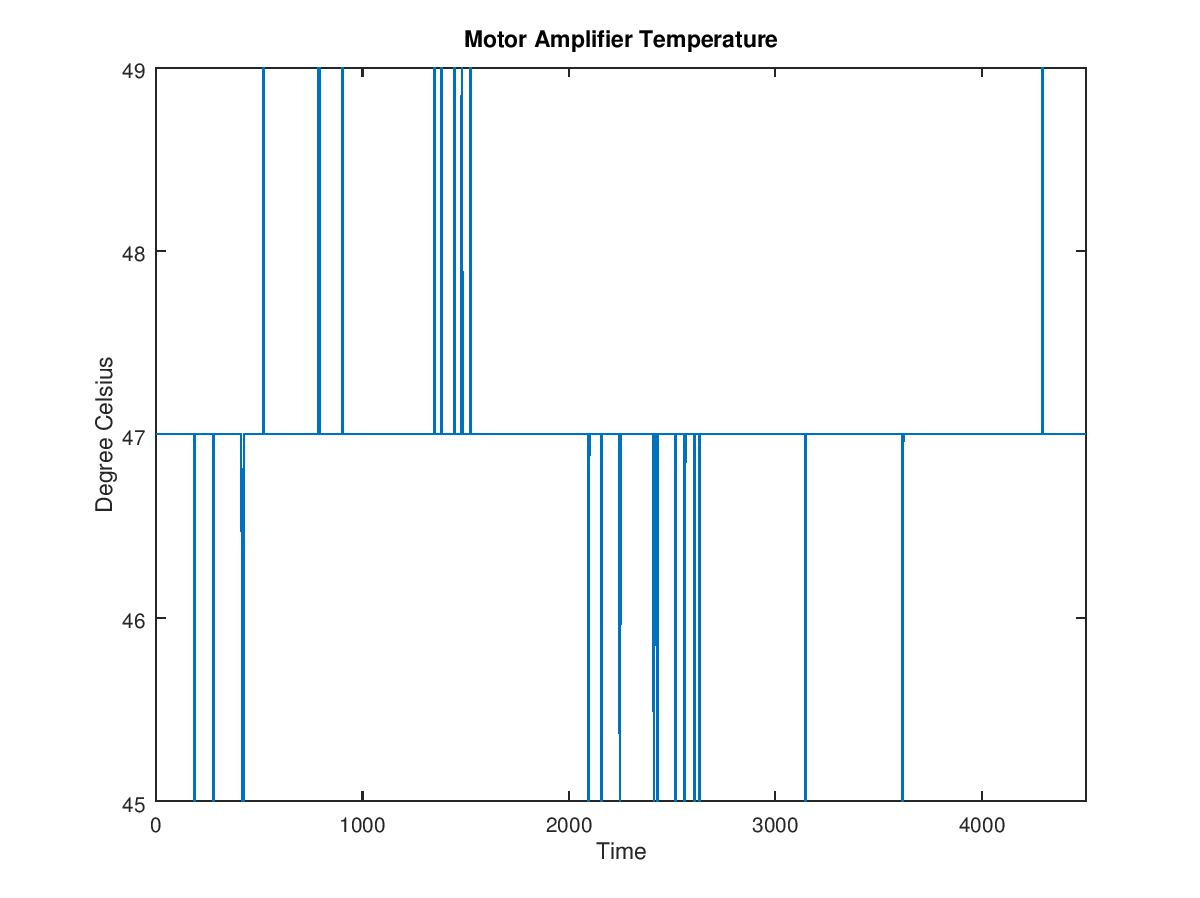
\includegraphics[width=.9\linewidth]{Figures/Motor_Amplifier_Temperature}
 \caption{Motor Amplifier Temperature}
 \label{fig:Motor Amplifier Temperature}
\end{subfigure}
\begin{subfigure}{.5\textwidth}
 \centering
 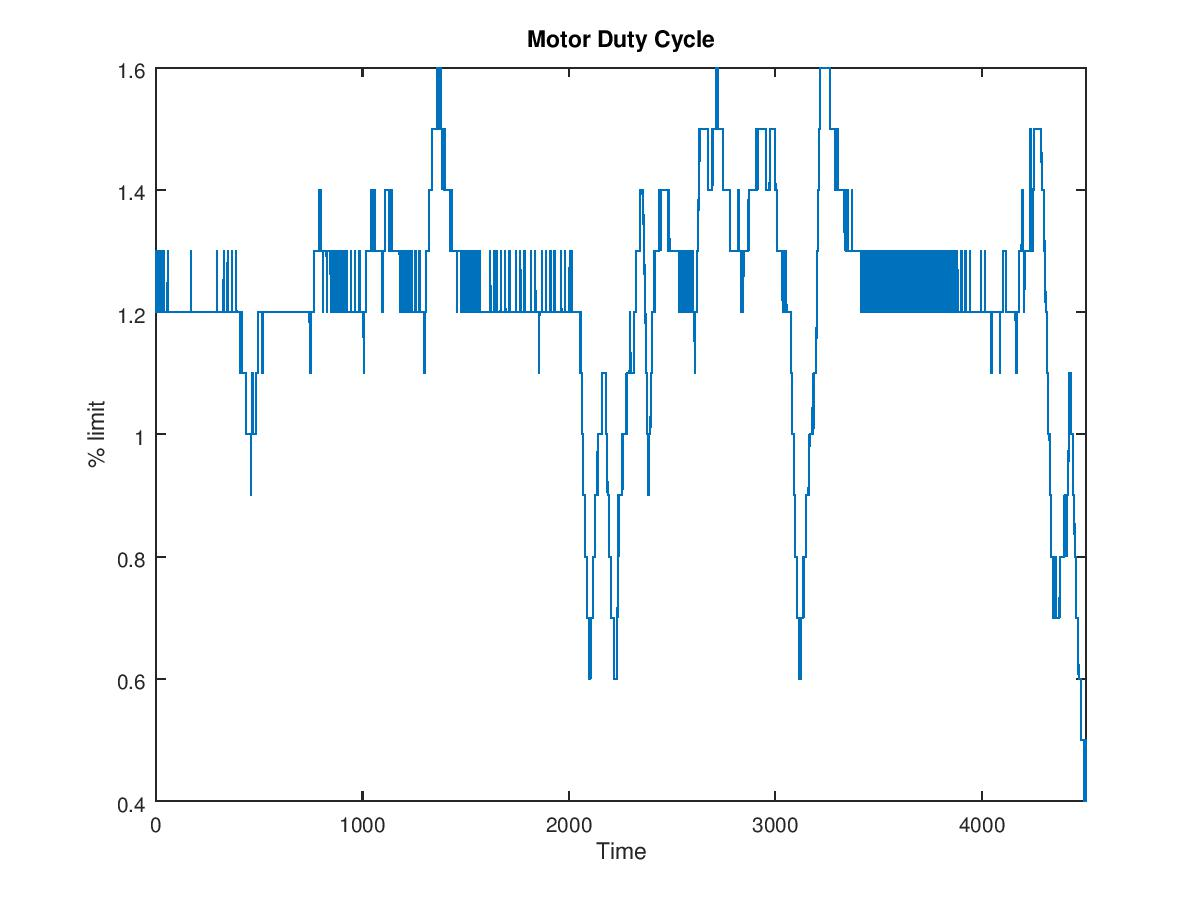
\includegraphics[width=.9\linewidth]{Figures/Motor_Duty_Cycle}
 \caption{Motor Duty cycle}
 \label{fig:Motor Duty Cycle}
\end{subfigure}
\caption[Data type plots]{Data type plots}
\label{fig:Data types}
\end{figure}

\subsubsection{Robot Bus Voltage}
\subsubsection{Robot AC input}
\subsubsection{Robot DC input}
\subsubsection{Robot Base board temperature}
\subsubsection{Motor Amplifier temperature}
\subsubsection{Motor Duty cycle}
\subsubsection{Motor Peak torque}
\subsubsection{Motor Peak velocity}
\subsubsection{Motor Peak position error}
